\section{Background}\label{sec:background} 
\begin{figure}[t]
  \centering
  \vspace{2mm}
  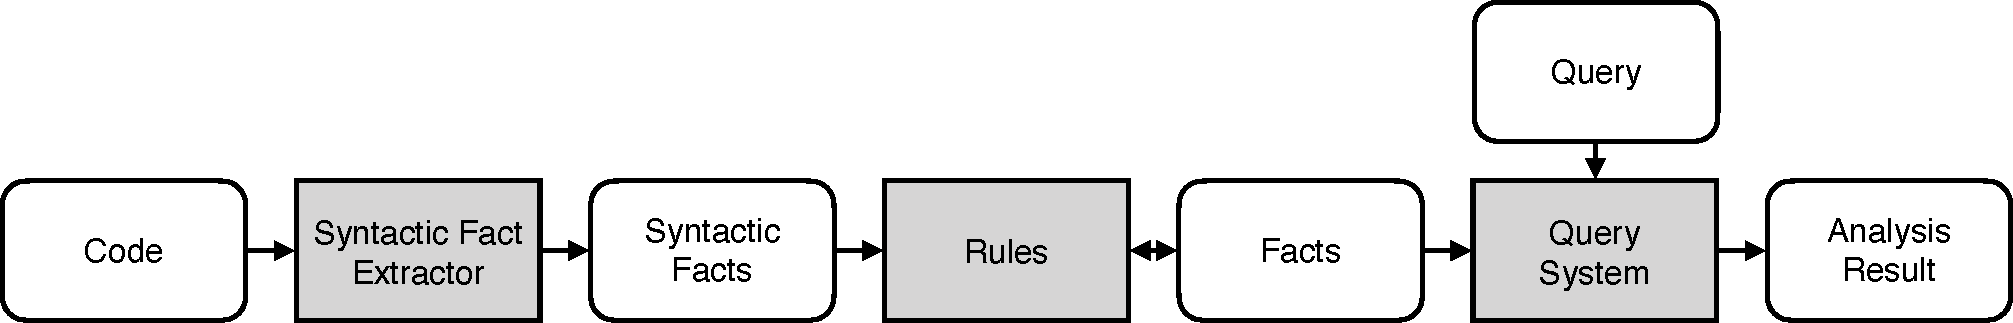
\includegraphics[width=0.47\textwidth]{img/ov1.pdf}
%  \vspace*{-1.5em}
  \caption{Overview of a declarative static analysis}
  \label{fig:ov1}
%\vspace*{-.5em}
\end{figure}

Figure~\ref{fig:ov1} presents the overview of how a declarative static
analysis works.  The analysis consists of three steps.  First, a given program
gets converted into syntactic facts.  Second, the rules that generate new facts
are defined, which correspond to the implementation of the analysis.  Finally,
the query system takes a query and evaluates the rules with the
given facts, producing an analysis result for the query.

%Figure~\ref{fig:ov1} presents the overview of how a declarative style analysis
%works. The analysis consists of three steps.  First, a given program gets
%converted into database of syntactic facts.  Second, the rules that generate
%new facts are defined, and a declarative language engine evaluates the rules
%with the given facts, producing new facts.  Finally, the query is executed to
%extract all the facts that meet certain conditions, which correspond to the
%analysis result.

\textbf{Step 1: Extracting syntactic facts.}
The first step is to extract syntactic facts from a given program source.
Syntactic facts include facts about certain AST nodes and
parent-child relationships between nodes. For example, consider
the following code:

\begin{lstlisting}[style=mcpp]
function f() {
  return 42;
}
\end{lstlisting}
We can define a syntactic fact of the form \rcode{ FunctionAt(ln, name)}, where
\rcode{ ln} denotes the line number and \rcode{ name} denotes the name of the function
defined at line \rcode{ ln}.  Therefore, we can extract the fact \rcode{
FunctionAt(1, "f")}.  Another example syntactic fact is \rcode{ EnclosingStmt(ln1,
ln2, i)}, which denotes that the function at line \rcode{ ln1} has the statement
at line \rcode{ ln2} as the \rcode{ i}-th statement in the function body.  For
example, we can extract the following syntactic fact: \rcode{ EnclosingStmt(1, 2,
0)}.

In a sense, these syntactic facts serve as building blocks for the
common Intermediate Representation (IR) of multiple languages.
Compared to other IRs, this declarative-style IR has a few advantages.
First, extracting information from source code in this format does not
require any understanding of the language semantics, which imposes
almost no performance overhead beyond parsing the source code.
Second, the syntactic facts can be utilized easily in other kinds of
analysis, since they are simple information that can be freely
manipulated when defining new rules. Therefore, even when we use a different
client analysis, we can reuse the extracted syntactic facts
without re-extracting them from the source code.

\smallskip
\textbf{Step 2: Defining rules.}
The next step is to define rules to generate new facts out of known facts.
 For example, we can define a dataflow
analysis \rcode{ Flow(x, z)},  which denotes that there is a dataflow from a node \rcode{ x}
to a node \rcode{ z}, where nodes represent program entities that can hold
run-time values, such as variables, literals, and function parameters.  We
can define a rule for this fact as the transitive closure of the fact named
\rcode{ Step}:

\begin{lstlisting}[style=mrule]
Flow(x, z) :- Step(x, z)
Flow(x, z) :- Step(x, y), Flow(y, z)
\end{lstlisting}

\noindent
where \rcode{ Step(x, z)} denotes a direct dataflow from \rcode{ x} to \rcode{ z}. The
rule derives a new fact \rcode{ Flow(x, z)} if there is a fact \rcode{ Step(x, z)} or
there are two facts \rcode{ Step(x, y)} and \rcode{ Flow(y, z)}.
The rules are usually
evaluated in a bottom-up and modular manner, that is, each rule is evaluated
one by one, after every rule it depends on is evaluated.

%The next step is to define rules to generate new facts out of known facts.
%%This step corresponds to actually implementing the algorithm of a
%%static analysis in a declarative style.
%For example, recall that we can define a call graph
%\rcode{ CallEdge(l1, l2)} using the facts
%named \rcode{ FunctionAt} and \rcode{ CallAt}.
%The defined rules are evaluated with declarative engines to finding all possible
%facts that can be derived. The rules are usually evaluated in a bottom-up
%and modular manner. Each rule is evaluated one-by-one, after every
%rule it depends on is evaluated. 

\smallskip
\textbf{Step 3: Performing queries.}
The final step is to perform the query via the query system.  A query consists
of a set of facts with variables, and the query system finds all variable
assignments that make every fact in that set can be derived. This step corresponds
to actually obtaining the final result of a static analysis in a declarative
style. 

%The final step is to perform queries via query system.
%The result of the query corresponds to actual result of client analysis.
%A query consists of set of facts, where some of the facts would have
%varaibles as arguments. Given a query, the query sytem will find all possible
%assignment on variables, that will make every facts would hold under
%the assignment.
